\documentclass[12pt]{article}

\usepackage{tikz,amsmath,amssymb}


\begin{document}


%\begin{tikzpicture}[scale=0.85]
% \tikzstyle{quadri}=[circle,draw,text=black, thick]
% \tikzstyle{estun}=[->,>=latex,very thick]
% \node[quadri] (R1) at (0,3) {$R_1$};
% \node[quadri] (R2) at (-2,1) {$R_2$};
% \node[quadri] (R3) at (0,1) {$R_3$};
% \node[quadri] (R4) at (2,1) {$R_4$};
% \node[quadri] (R5) at (0,-1) {$R_5$};
% \node[quadri] (R6) at (1.5,-1) {$R_6$};
% \node[quadri] (R7) at (2.5,-1) {$R_7$};
% \node[quadri] (R8) at (4,3) {$R_8$};
% \node[quadri] (R9) at (4,1) {$R_9$};
% \draw[estun] (R1)--(R2);
% \draw[estun] (R1)--(R3);
% \draw[estun] (R1)--(R4);
% \draw[estun] (R3)--(R5);
% \draw[estun] (R4)--(R6);
% \draw[estun] (R4)--(R7);
% \draw[estun] (R8)--(R9);
%\end{tikzpicture}

Brouillon :

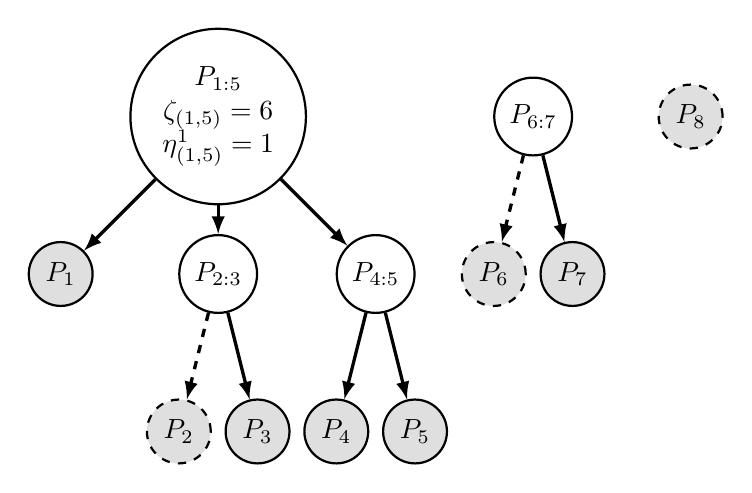
\begin{tikzpicture}[scale=1]
 \tikzstyle{quadri}=[circle,draw,text=black,thick]
 \tikzstyle{estun}=[->,>=latex,very thick]
 %
 \node[quadri, align=center] (P15) at (0,3) {$P_{1:5}$\\ $\zeta_{(1,5)}=6$ \\ $\eta_{(1,5)}^1=1$};
 \node[quadri, fill=gray!25] (P1) at (-2,1) {$P_1$};
 \node[quadri] (P23) at (0,1) {$P_{2:3}$};
 \node[quadri] (P45) at (2,1) {$P_{4:5}$};
 \node[quadri, dashed,fill=gray!25] (P2) at (-0.5,-1) {$P_2$};
 \node[quadri,fill=gray!25] (P3) at (0.5,-1) {$P_3$};
 \node[quadri,fill=gray!25] (P4) at (1.5,-1) {$P_4$};
 \node[quadri,fill=gray!25] (P5) at (2.5,-1) {$P_5$};
 \node[quadri] (P67) at (4,3) {$P_{6:7}$};
 \node[quadri,dashed,fill=gray!25] (P6) at (3.5,1) {$P_6$};
 \node[quadri,fill=gray!25] (P7) at (4.5,1) {$P_7$};
 \node[quadri,dashed,fill=gray!25] (P8) at (6,3) {$P_8$};
 %
 \draw[estun] (P15)--(P1);
 \draw[estun] (P15)--(P23);
 \draw[estun] (P15)--(P45);
 \draw[estun] (P23)--(P3);
 \draw[estun,dashed] (P23)--(P2);
 \draw[estun] (P45)--(P4);
 \draw[estun] (P45)--(P5);
 \draw[estun] (P67)--(P7);
 \draw[estun,dashed] (P67)--(P6);
\end{tikzpicture}

Première figure avec les zetas avant pruning :

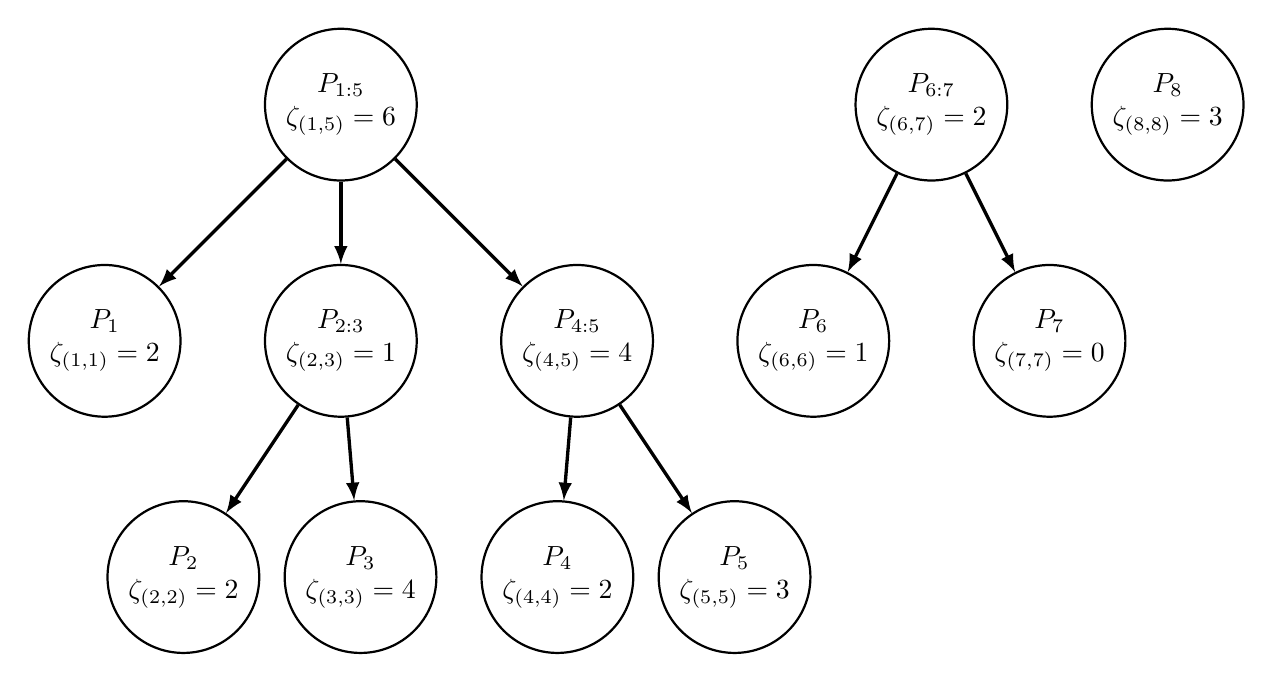
\begin{tikzpicture}[scale=1]
 \tikzstyle{quadri}=[circle, draw, text=black, thick, align=center]
 \tikzstyle{estun}=[->, >=latex, very thick]
 %
 \node[quadri] (P15) at (0, 3) {$P_{1:5}$\\$\zeta_{(1, 5)}=6$};
 \node[quadri] (P67) at (7.5, 3) {$P_{6:7}$\\$\zeta_{(6, 7)}=2$};
 \node[quadri] (P8) at (10.5, 3) {$P_8$\\$\zeta_{(8, 8)}=3$};
 %
 \node[quadri] (P1) at (-3, 0) {$P_1$\\$\zeta_{(1, 1)}=2$};
 \node[quadri] (P23) at (0, 0) {$P_{2:3}$\\$\zeta_{(2, 3)}=1$};
 \node[quadri] (P45) at (3, 0) {$P_{4:5}$\\$\zeta_{(4, 5)}=4$};
 \node[quadri] (P6) at (6, 0) {$P_6$\\$\zeta_{(6, 6)}=1$};
 \node[quadri] (P7) at (9, 0) {$P_7$\\$\zeta_{(7, 7)}=0$};
 %
 \node[quadri] (P2) at (-2, -3) {$P_2$\\$\zeta_{(2, 2)}=2$};
 \node[quadri] (P3) at (0.25, -3) {$P_3$\\$\zeta_{(3, 3)}=4$};
 \node[quadri] (P4) at (2.75, -3) {$P_4$\\$\zeta_{(4, 4)}=2$};
 \node[quadri] (P5) at (5, -3) {$P_5$\\$\zeta_{(5, 5)}=3$};
 %%
 \draw[estun] (P15)--(P1);
 \draw[estun] (P15)--(P23);
 \draw[estun] (P15)--(P45);
 \draw[estun] (P23)--(P3);
 \draw[estun] (P23)--(P2);
 \draw[estun] (P45)--(P4);
 \draw[estun] (P45)--(P5);
 \draw[estun] (P67)--(P7);
 \draw[estun] (P67)--(P6);
\end{tikzpicture}


Deuxième figure avec les zetas après pruning, sans les zeta :

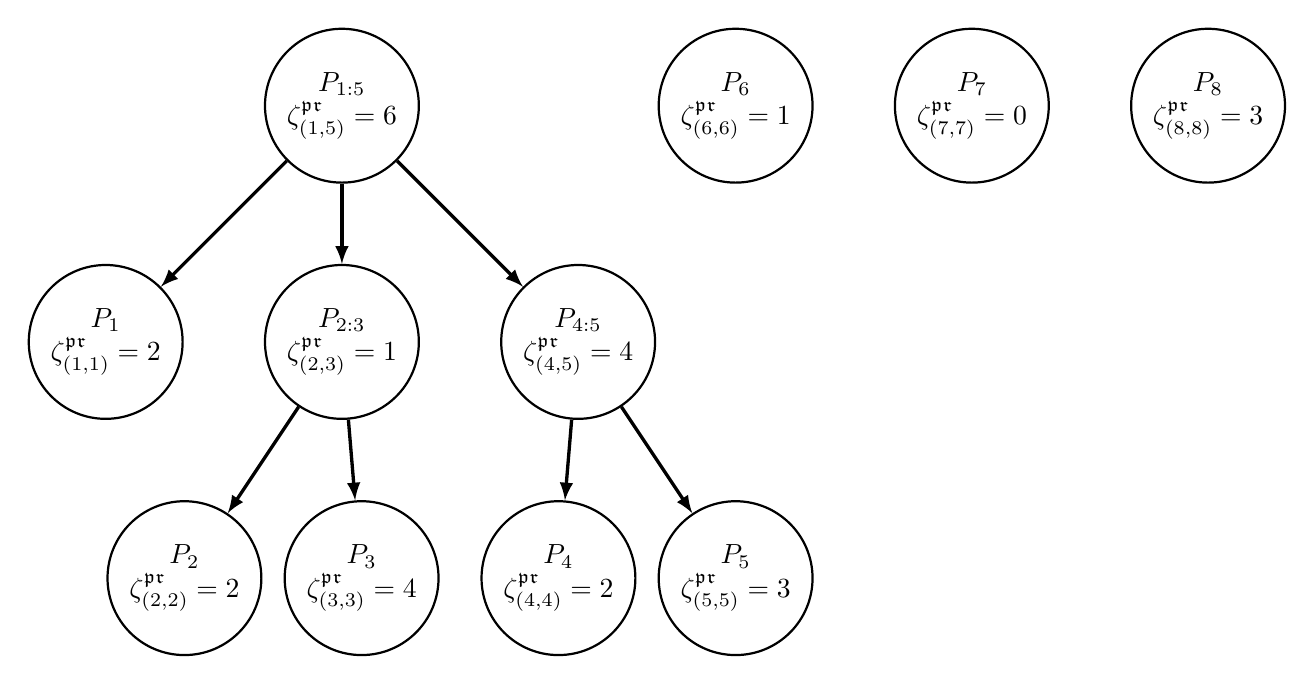
\begin{tikzpicture}[scale=1]
 \tikzstyle{quadri}=[circle, draw, text=black, thick, align=center]
 \tikzstyle{estun}=[->, >=latex, very thick]
 %
 \node[quadri] (P15) at (0, 3) {$P_{1:5}$\\$\zeta^{\mathfrak{pr}}_{(1, 5)}=6$};
 \node[quadri] (P8) at (11, 3) {$P_8$\\$\zeta^{\mathfrak{pr}}_{(8, 8)}=3$};
 %
 \node[quadri] (P1) at (-3, 0) {$P_1$\\$\zeta^{\mathfrak{pr}}_{(1, 1)}=2$};
 \node[quadri] (P23) at (0, 0) {$P_{2:3}$\\$\zeta^{\mathfrak{pr}}_{(2, 3)}=1$};
 \node[quadri] (P45) at (3, 0) {$P_{4:5}$\\$\zeta^{\mathfrak{pr}}_{(4, 5)}=4$};
 \node[quadri] (P6) at (5, 3) {$P_6$\\$\zeta^{\mathfrak{pr}}_{(6, 6)}=1$};
 \node[quadri] (P7) at (8, 3) {$P_7$\\$\zeta^{\mathfrak{pr}}_{(7, 7)}=0$};
 %
 \node[quadri] (P2) at (-2, -3) {$P_2$\\$\zeta^{\mathfrak{pr}}_{(2, 2)}=2$};
 \node[quadri] (P3) at (0.25, -3) {$P_3$\\$\zeta^{\mathfrak{pr}}_{(3, 3)}=4$};
 \node[quadri] (P4) at (2.75, -3) {$P_4$\\$\zeta^{\mathfrak{pr}}_{(4, 4)}=2$};
 \node[quadri] (P5) at (5, -3) {$P_5$\\$\zeta^{\mathfrak{pr}}_{(5, 5)}=3$};
 %%
 \draw[estun] (P15)--(P1);
 \draw[estun] (P15)--(P23);
 \draw[estun] (P15)--(P45);
 \draw[estun] (P23)--(P3);
 \draw[estun] (P23)--(P2);
 \draw[estun] (P45)--(P4);
 \draw[estun] (P45)--(P5);
\end{tikzpicture}

Deuxième.5 figure avec les zetas après pruning, les zeta initialisés à 0 :

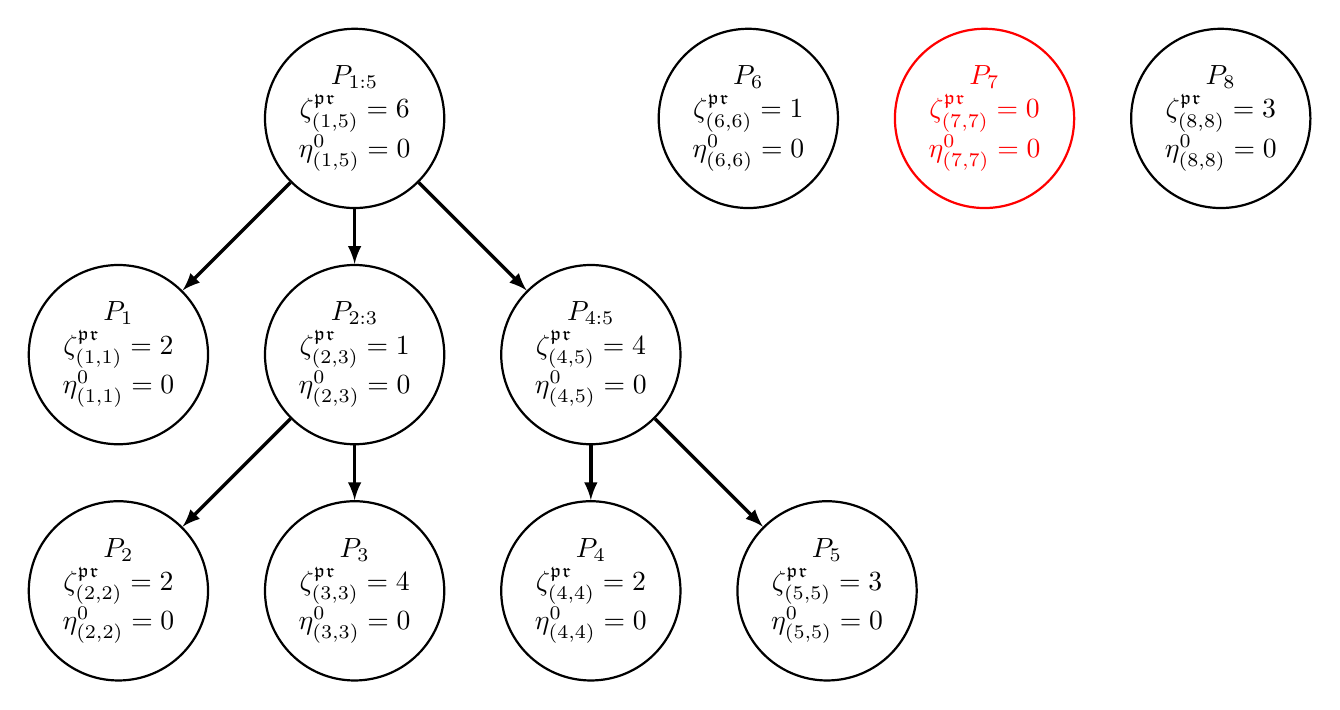
\begin{tikzpicture}[scale=1]
 \tikzstyle{quadri}=[circle, draw, text=black, thick, align=center]
 \tikzstyle{estun}=[->, >=latex, very thick]
 %
 \node[quadri] (P15) at (0, 3) {$P_{1:5}$\\$\zeta^{\mathfrak{pr}}_{(1, 5)}=6$\\$\eta_{(1, 5)}^0=0$};
 \node[quadri] (P8) at (11, 3) {$P_8$\\$\zeta^{\mathfrak{pr}}_{(8, 8)}=3$\\$\eta_{(8, 8)}^0=0$};
 %
 \node[quadri] (P1) at (-3, 0) {$P_1$\\$\zeta^{\mathfrak{pr}}_{(1, 1)}=2$\\$\eta_{(1, 1)}^0=0$};
 \node[quadri] (P23) at (0, 0) {$P_{2:3}$\\$\zeta^{\mathfrak{pr}}_{(2, 3)}=1$\\$\eta_{(2, 3)}^0=0$};
 \node[quadri] (P45) at (3, 0) {$P_{4:5}$\\$\zeta^{\mathfrak{pr}}_{(4, 5)}=4$\\$\eta_{(4, 5)}^0=0$};
 \node[quadri] (P6) at (5, 3) {$P_6$\\$\zeta^{\mathfrak{pr}}_{(6, 6)}=1$\\$\eta_{(6, 6)}^0=0$};
 \node[quadri, red] (P7) at (8, 3) {$P_7$\\$\zeta^{\mathfrak{pr}}_{(7, 7)}=0$\\$\eta_{(7, 7)}^0=0$};
 %
 \node[quadri] (P2) at (-3, -3) {$P_2$\\$\zeta^{\mathfrak{pr}}_{(2, 2)}=2$\\$\eta_{(2, 2)}^0=0$};
 \node[quadri] (P3) at (-0, -3) {$P_3$\\$\zeta^{\mathfrak{pr}}_{(3, 3)}=4$\\$\eta_{(3, 3)}^0=0$};
 \node[quadri] (P4) at (3, -3) {$P_4$\\$\zeta^{\mathfrak{pr}}_{(4, 4)}=2$\\$\eta_{(4, 4)}^0=0$};
 \node[quadri] (P5) at (6, -3) {$P_5$\\$\zeta^{\mathfrak{pr}}_{(5, 5)}=3$\\$\eta_{(5, 5)}^0=0$};
 %%
 \draw[estun] (P15)--(P1);
 \draw[estun] (P15)--(P23);
 \draw[estun] (P15)--(P45);
 \draw[estun] (P23)--(P3);
 \draw[estun] (P23)--(P2);
 \draw[estun] (P45)--(P4);
 \draw[estun] (P45)--(P5);
\end{tikzpicture}

Troisième figure avec $i_1=11$

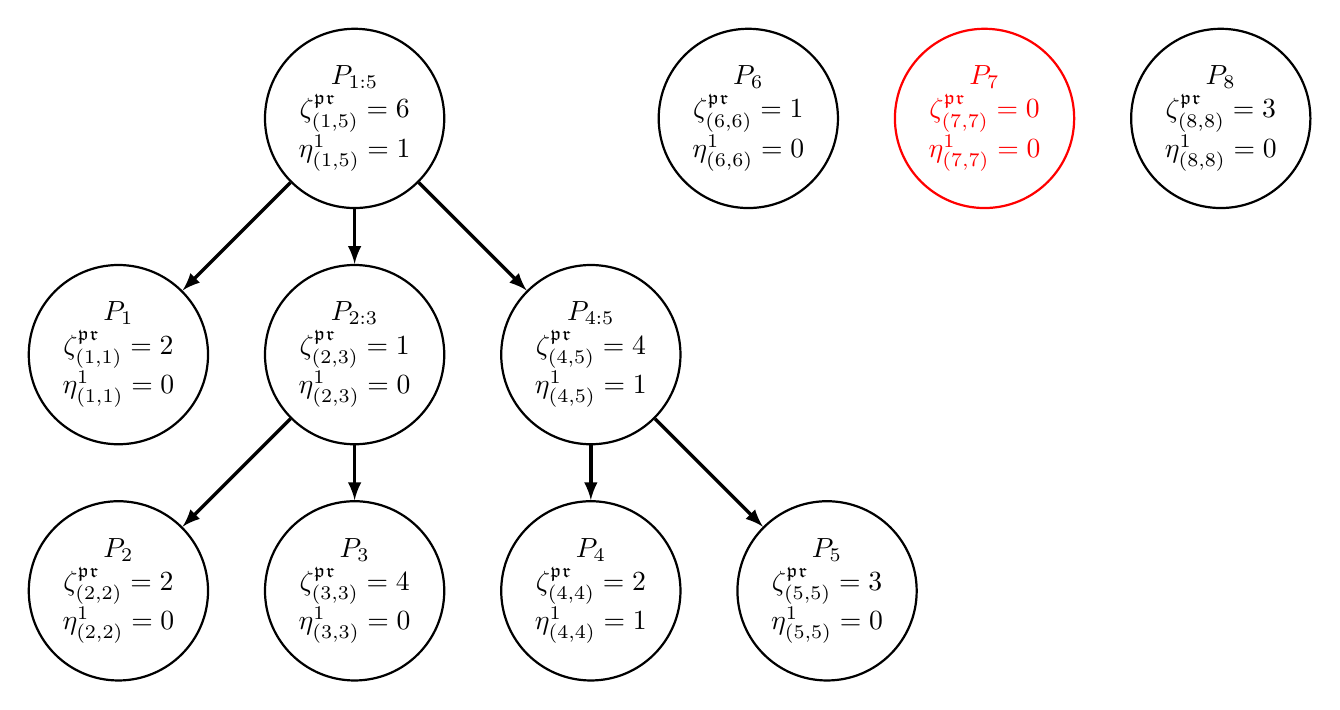
\begin{tikzpicture}[scale=1]
 \tikzstyle{quadri}=[circle, draw, text=black, thick, align=center]
 \tikzstyle{estun}=[->, >=latex, very thick]
 %
 \node[quadri] (P15) at (0, 3) {$P_{1:5}$\\$\zeta^{\mathfrak{pr}}_{(1, 5)}=6$\\$\eta_{(1, 5)}^1=1$};
 \node[quadri] (P8) at (11, 3) {$P_8$\\$\zeta^{\mathfrak{pr}}_{(8, 8)}=3$\\$\eta_{(8, 8)}^1=0$};
 %
 \node[quadri] (P1) at (-3, 0) {$P_1$\\$\zeta^{\mathfrak{pr}}_{(1, 1)}=2$\\$\eta_{(1, 1)}^1=0$};
 \node[quadri] (P23) at (0, 0) {$P_{2:3}$\\$\zeta^{\mathfrak{pr}}_{(2, 3)}=1$\\$\eta_{(2, 3)}^1=0$};
 \node[quadri] (P45) at (3, 0) {$P_{4:5}$\\$\zeta^{\mathfrak{pr}}_{(4, 5)}=4$\\$\eta_{(4, 5)}^1=1$};
 \node[quadri] (P6) at (5, 3) {$P_6$\\$\zeta^{\mathfrak{pr}}_{(6, 6)}=1$\\$\eta_{(6, 6)}^1=0$};
 \node[quadri, red] (P7) at (8, 3) {$P_7$\\$\zeta^{\mathfrak{pr}}_{(7, 7)}=0$\\$\eta_{(7, 7)}^1=0$};
 %
 \node[quadri] (P2) at (-3, -3) {$P_2$\\$\zeta^{\mathfrak{pr}}_{(2, 2)}=2$\\$\eta_{(2, 2)}^1=0$};
 \node[quadri] (P3) at (-0, -3) {$P_3$\\$\zeta^{\mathfrak{pr}}_{(3, 3)}=4$\\$\eta_{(3, 3)}^1=0$};
 \node[quadri] (P4) at (3, -3) {$P_4$\\$\zeta^{\mathfrak{pr}}_{(4, 4)}=2$\\$\eta_{(4, 4)}^1=1$};
 \node[quadri] (P5) at (6, -3) {$P_5$\\$\zeta^{\mathfrak{pr}}_{(5, 5)}=3$\\$\eta_{(5, 5)}^1=0$};
 %%
 \draw[estun] (P15)--(P1);
 \draw[estun] (P15)--(P23);
 \draw[estun] (P15)--(P45);
 \draw[estun] (P23)--(P3);
 \draw[estun] (P23)--(P2);
 \draw[estun] (P45)--(P4);
 \draw[estun] (P45)--(P5);
\end{tikzpicture}

Quatrième figure avec $i_2=17$

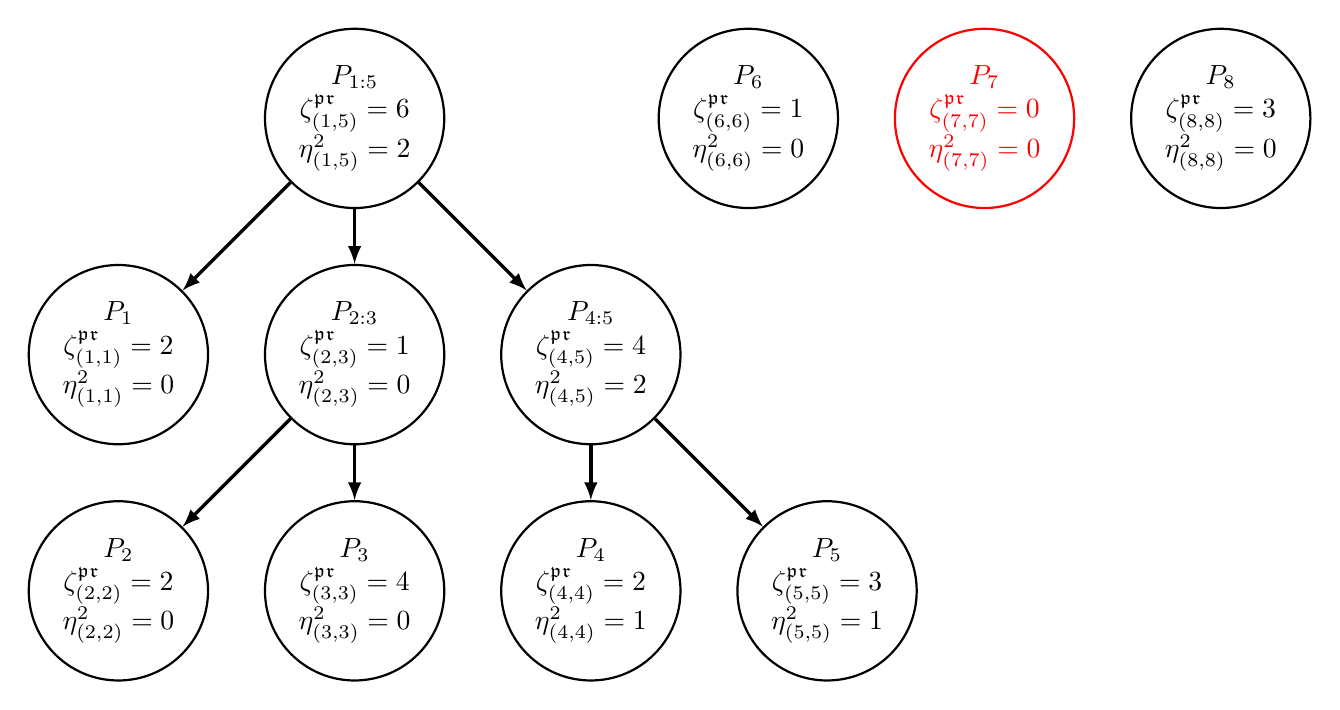
\begin{tikzpicture}[scale=1]
 \tikzstyle{quadri}=[circle, draw, text=black, thick, align=center]
 \tikzstyle{estun}=[->, >=latex, very thick]
 %
 \node[quadri] (P15) at (0, 3) {$P_{1:5}$\\$\zeta^{\mathfrak{pr}}_{(1, 5)}=6$\\$\eta_{(1, 5)}^2=2$};
 \node[quadri] (P8) at (11, 3) {$P_8$\\$\zeta^{\mathfrak{pr}}_{(8, 8)}=3$\\$\eta_{(8, 8)}^2=0$};
 %
 \node[quadri] (P1) at (-3, 0) {$P_1$\\$\zeta^{\mathfrak{pr}}_{(1, 1)}=2$\\$\eta_{(1, 1)}^2=0$};
 \node[quadri] (P23) at (0, 0) {$P_{2:3}$\\$\zeta^{\mathfrak{pr}}_{(2, 3)}=1$\\$\eta_{(2, 3)}^2=0$};
 \node[quadri] (P45) at (3, 0) {$P_{4:5}$\\$\zeta^{\mathfrak{pr}}_{(4, 5)}=4$\\$\eta_{(4, 5)}^2=2$};
 \node[quadri] (P6) at (5, 3) {$P_6$\\$\zeta^{\mathfrak{pr}}_{(6, 6)}=1$\\$\eta_{(6, 6)}^2=0$};
 \node[quadri, red] (P7) at (8, 3) {$P_7$\\$\zeta^{\mathfrak{pr}}_{(7, 7)}=0$\\$\eta_{(7, 7)}^2=0$};
 %
 \node[quadri] (P2) at (-3, -3) {$P_2$\\$\zeta^{\mathfrak{pr}}_{(2, 2)}=2$\\$\eta_{(2, 2)}^2=0$};
 \node[quadri] (P3) at (-0, -3) {$P_3$\\$\zeta^{\mathfrak{pr}}_{(3, 3)}=4$\\$\eta_{(3, 3)}^2=0$};
 \node[quadri] (P4) at (3, -3) {$P_4$\\$\zeta^{\mathfrak{pr}}_{(4, 4)}=2$\\$\eta_{(4, 4)}^2=1$};
 \node[quadri] (P5) at (6, -3) {$P_5$\\$\zeta^{\mathfrak{pr}}_{(5, 5)}=3$\\$\eta_{(5, 5)}^2=1$};
 %%
 \draw[estun] (P15)--(P1);
 \draw[estun] (P15)--(P23);
 \draw[estun] (P15)--(P45);
 \draw[estun] (P23)--(P3);
 \draw[estun] (P23)--(P2);
 \draw[estun] (P45)--(P4);
 \draw[estun] (P45)--(P5);
\end{tikzpicture}

Quatrième figure avec $i_3=12$

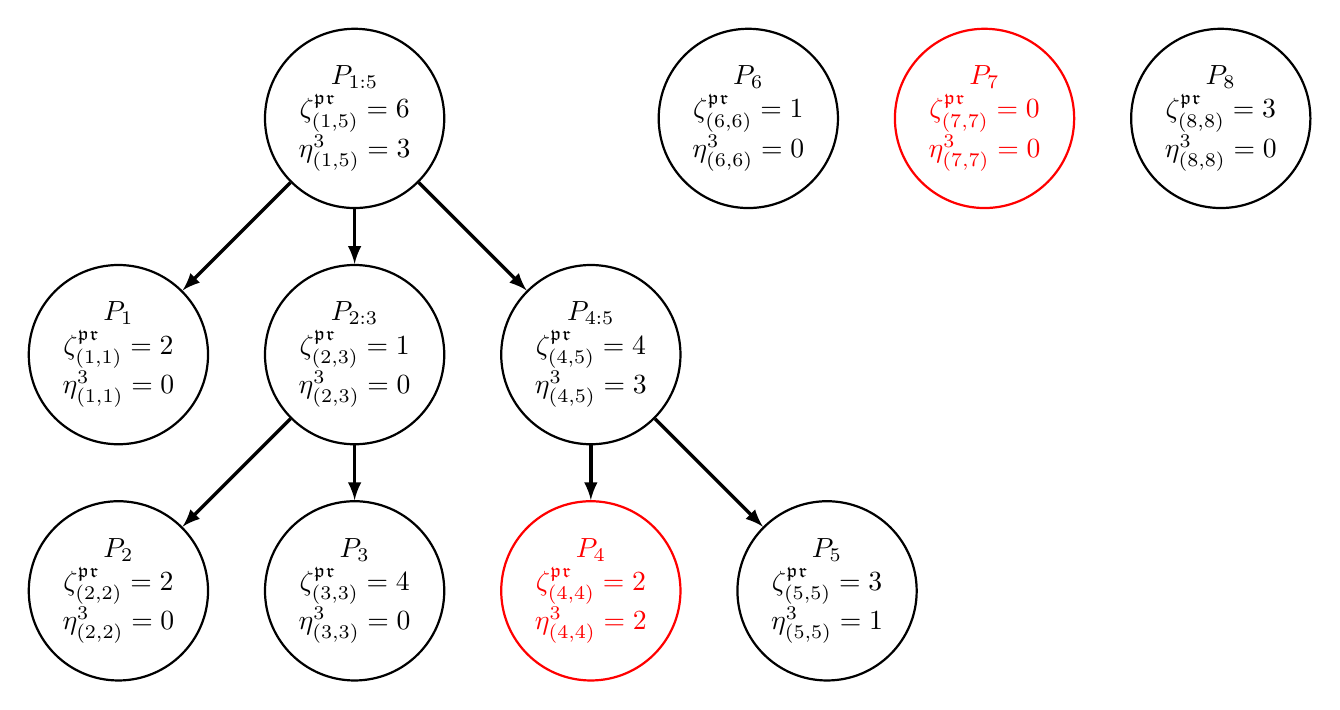
\begin{tikzpicture}[scale=1]
 \tikzstyle{quadri}=[circle, draw, text=black, thick, align=center]
 \tikzstyle{estun}=[->, >=latex, very thick]
 %
 \node[quadri] (P15) at (0, 3) {$P_{1:5}$\\$\zeta^{\mathfrak{pr}}_{(1, 5)}=6$\\$\eta_{(1, 5)}^3=3$};
 \node[quadri] (P8) at (11, 3) {$P_8$\\$\zeta^{\mathfrak{pr}}_{(8, 8)}=3$\\$\eta_{(8, 8)}^3=0$};
 %
 \node[quadri] (P1) at (-3, 0) {$P_1$\\$\zeta^{\mathfrak{pr}}_{(1, 1)}=2$\\$\eta_{(1, 1)}^3=0$};
 \node[quadri] (P23) at (0, 0) {$P_{2:3}$\\$\zeta^{\mathfrak{pr}}_{(2, 3)}=1$\\$\eta_{(2, 3)}^3=0$};
 \node[quadri] (P45) at (3, 0) {$P_{4:5}$\\$\zeta^{\mathfrak{pr}}_{(4, 5)}=4$\\$\eta_{(4, 5)}^3=3$};
 \node[quadri] (P6) at (5, 3) {$P_6$\\$\zeta^{\mathfrak{pr}}_{(6, 6)}=1$\\$\eta_{(6, 6)}^3=0$};
 \node[quadri, red] (P7) at (8, 3) {$P_7$\\$\zeta^{\mathfrak{pr}}_{(7, 7)}=0$\\$\eta_{(7, 7)}^3=0$};
 %
 \node[quadri] (P2) at (-3, -3) {$P_2$\\$\zeta^{\mathfrak{pr}}_{(2, 2)}=2$\\$\eta_{(2, 2)}^3=0$};
 \node[quadri] (P3) at (-0, -3) {$P_3$\\$\zeta^{\mathfrak{pr}}_{(3, 3)}=4$\\$\eta_{(3, 3)}^3=0$};
 \node[quadri, red] (P4) at (3, -3) {$P_4$\\$\zeta^{\mathfrak{pr}}_{(4, 4)}=2$\\$\eta_{(4, 4)}^3=2$};
 \node[quadri] (P5) at (6, -3) {$P_5$\\$\zeta^{\mathfrak{pr}}_{(5, 5)}=3$\\$\eta_{(5, 5)}^3=1$};
 %%
 \draw[estun] (P15)--(P1);
 \draw[estun] (P15)--(P23);
 \draw[estun] (P15)--(P45);
 \draw[estun] (P23)--(P3);
 \draw[estun] (P23)--(P2);
 \draw[estun] (P45)--(P4);
 \draw[estun] (P45)--(P5);
\end{tikzpicture}

$i_4=13\in P_4 \subseteq  \bigcup_{k\in \mathcal{K}^-_3} R_k$ donc on ne fait rien et on maintient tous les $\eta_k^4=\eta_k^3$ (ligne 9)

Cinquième figure avec $i_5=18$, on ne met pas à jour $\eta_{(5, 5)}^5$ car on s'est arrêté avant (ligne 23)

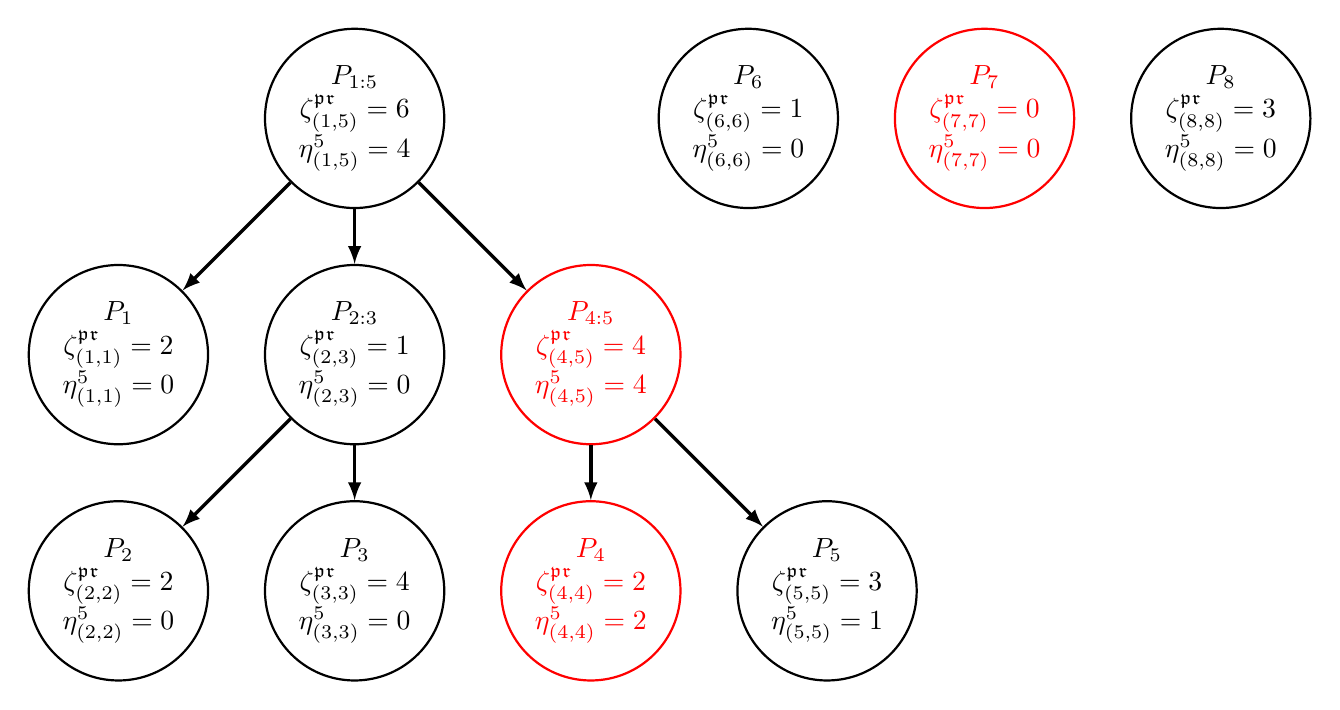
\begin{tikzpicture}[scale=1]
 \tikzstyle{quadri}=[circle, draw, text=black, thick, align=center]
 \tikzstyle{estun}=[->, >=latex, very thick]
 %
 \node[quadri] (P15) at (0, 3) {$P_{1:5}$\\$\zeta^{\mathfrak{pr}}_{(1, 5)}=6$\\$\eta_{(1, 5)}^5=4$};
 \node[quadri] (P8) at (11, 3) {$P_8$\\$\zeta^{\mathfrak{pr}}_{(8, 8)}=3$\\$\eta_{(8, 8)}^5=0$};
 %
 \node[quadri] (P1) at (-3, 0) {$P_1$\\$\zeta^{\mathfrak{pr}}_{(1, 1)}=2$\\$\eta_{(1, 1)}^5=0$};
 \node[quadri] (P23) at (0, 0) {$P_{2:3}$\\$\zeta^{\mathfrak{pr}}_{(2, 3)}=1$\\$\eta_{(2, 3)}^5=0$};
 \node[quadri, red] (P45) at (3, 0) {$P_{4:5}$\\$\zeta^{\mathfrak{pr}}_{(4, 5)}=4$\\$\eta_{(4, 5)}^5=4$};
 \node[quadri] (P6) at (5, 3) {$P_6$\\$\zeta^{\mathfrak{pr}}_{(6, 6)}=1$\\$\eta_{(6, 6)}^5=0$};
 \node[quadri, red] (P7) at (8, 3) {$P_7$\\$\zeta^{\mathfrak{pr}}_{(7, 7)}=0$\\$\eta_{(7, 7)}^5=0$};
 %
 \node[quadri] (P2) at (-3, -3) {$P_2$\\$\zeta^{\mathfrak{pr}}_{(2, 2)}=2$\\$\eta_{(2, 2)}^5=0$};
 \node[quadri] (P3) at (-0, -3) {$P_3$\\$\zeta^{\mathfrak{pr}}_{(3, 3)}=4$\\$\eta_{(3, 3)}^5=0$};
 \node[quadri, red] (P4) at (3, -3) {$P_4$\\$\zeta^{\mathfrak{pr}}_{(4, 4)}=2$\\$\eta_{(4, 4)}^5=2$};
 \node[quadri] (P5) at (6, -3) {$P_5$\\$\zeta^{\mathfrak{pr}}_{(5, 5)}=3$\\$\eta_{(5, 5)}^5=1$};
 %%
 \draw[estun] (P15)--(P1);
 \draw[estun] (P15)--(P23);
 \draw[estun] (P15)--(P45);
 \draw[estun] (P23)--(P3);
 \draw[estun] (P23)--(P2);
 \draw[estun] (P45)--(P4);
 \draw[estun] (P45)--(P5);
\end{tikzpicture}

Sixième figure avec $i_6=3$, on ne met pas à jour $\eta_{(2, 2)}^6$ car on s'est arrêté avant (ligne 23)

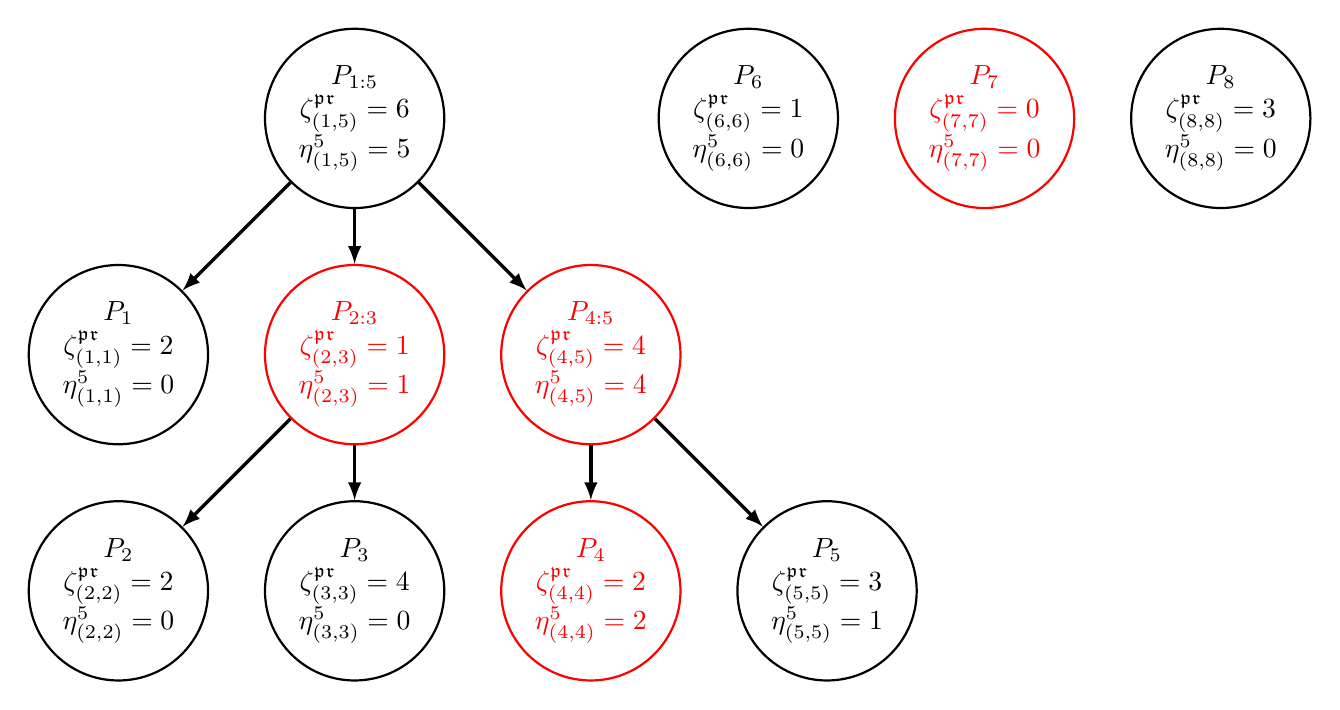
\begin{tikzpicture}[scale=1]
 \tikzstyle{quadri}=[circle, draw, text=black, thick, align=center]
 \tikzstyle{estun}=[->, >=latex, very thick]
 %
 \node[quadri] (P15) at (0, 3) {$P_{1:5}$\\$\zeta^{\mathfrak{pr}}_{(1, 5)}=6$\\$\eta_{(1, 5)}^5=5$};
 \node[quadri] (P8) at (11, 3) {$P_8$\\$\zeta^{\mathfrak{pr}}_{(8, 8)}=3$\\$\eta_{(8, 8)}^5=0$};
 %
 \node[quadri] (P1) at (-3, 0) {$P_1$\\$\zeta^{\mathfrak{pr}}_{(1, 1)}=2$\\$\eta_{(1, 1)}^5=0$};
 \node[quadri, red] (P23) at (0, 0) {$P_{2:3}$\\$\zeta^{\mathfrak{pr}}_{(2, 3)}=1$\\$\eta_{(2, 3)}^5=1$};
 \node[quadri, red] (P45) at (3, 0) {$P_{4:5}$\\$\zeta^{\mathfrak{pr}}_{(4, 5)}=4$\\$\eta_{(4, 5)}^5=4$};
 \node[quadri] (P6) at (5, 3) {$P_6$\\$\zeta^{\mathfrak{pr}}_{(6, 6)}=1$\\$\eta_{(6, 6)}^5=0$};
 \node[quadri, red] (P7) at (8, 3) {$P_7$\\$\zeta^{\mathfrak{pr}}_{(7, 7)}=0$\\$\eta_{(7, 7)}^5=0$};
 %
 \node[quadri] (P2) at (-3, -3) {$P_2$\\$\zeta^{\mathfrak{pr}}_{(2, 2)}=2$\\$\eta_{(2, 2)}^5=0$};
 \node[quadri] (P3) at (-0, -3) {$P_3$\\$\zeta^{\mathfrak{pr}}_{(3, 3)}=4$\\$\eta_{(3, 3)}^5=0$};
 \node[quadri, red] (P4) at (3, -3) {$P_4$\\$\zeta^{\mathfrak{pr}}_{(4, 4)}=2$\\$\eta_{(4, 4)}^5=2$};
 \node[quadri] (P5) at (6, -3) {$P_5$\\$\zeta^{\mathfrak{pr}}_{(5, 5)}=3$\\$\eta_{(5, 5)}^5=1$};
 %%
 \draw[estun] (P15)--(P1);
 \draw[estun] (P15)--(P23);
 \draw[estun] (P15)--(P45);
 \draw[estun] (P23)--(P3);
 \draw[estun] (P23)--(P2);
 \draw[estun] (P45)--(P4);
 \draw[estun] (P45)--(P5);
\end{tikzpicture}



\end{document}
